\documentclass[UTF8,11pt]{ctexart}
\usepackage{amsthm} % theorems
\usepackage{amsfonts} % mathbb
\usepackage{amsmath} % bmatrix
\usepackage{graphicx} % figure
\usepackage{geometry}
\geometry{scale=0.8}

\title{数学分析与线性代数例题}
\author{佚名}
\date{\today}

\newtheorem{theorem}{定理}
\newtheorem{example}{例}
\newtheorem*{answer}{解}

\begin{document}

\maketitle
\tableofcontents

\section{微分中值定理及其应用}
\begin{theorem}[极值的第二充分条件]
设 $f(x)$ 在 $(x_0-\delta,x_0+\delta)$ 可导且 $f'(x_0)=0$,又 $f''(x_0)$ 存在.
\begin{itemize}
	\item [1)] 若 $f''(x_0)<0$ ,则 $f(x_0)$ 是严格极大值;
	\item [2)] 若 $f''(x_0)>0$ ,则 $f(x_0)$ 是严格极小值.
\end{itemize}
\end{theorem}

\begin{example}
求 $y=\frac{1}{3}x\sqrt[3]{(x-5)^2}$ 的极值点与极值\footnote{原题摘自《数学分析简明教程》(上册)P142.}.
\end{example}
\begin{answer}
函数在 $(-\infty,+\infty)$ 上连续,当 $x\ne 5$ 时有
\begin{equation}
y'=\frac{1}{3}\left((x-5)^\frac{2}{3}+\frac{2x}{3}(x-5)^{-\frac{1}{3}}\right)
=\frac{5(x-3)}{9(x-5)^{1/3}}\,.
\end{equation}
令 $y'=0$ 得稳定点 $x=3$,现列表如下:
\begin{center}
\begin{tabular}{|c|c|c|c|c|c|}\hline
$x$ & $(-\infty,3)$ & $3$ & $(3,5)$ & $5$ & $(5,+\infty)$ \\\hline
$y'$ & $+$ & $0$ & $-$ & 不存在 & $+$\\\hline
$y$ & $\nearrow$ & $\sqrt[3]{4}$ & $\searrow$ & $0$ & $\nearrow$\\\hline
\end{tabular}
\end{center}

从表中可见 $x=3$ 是极大值点,极大值为 $f(3)=\sqrt[3]{4}$;$x=5$ 为极小值点,极小值为 $f(5)=0$.
我们可以大致地画出函数的图形,如图\ref{fig:function}所示.
\begin{figure}[htbp]
\centering
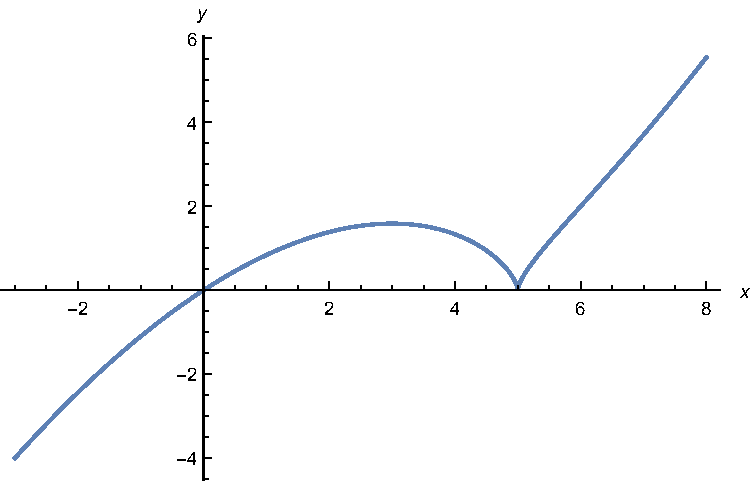
\includegraphics[width=0.5\linewidth]{fig/function.pdf}
\caption{$y=\frac{1}{3}x\sqrt[3]{(x-5)^2}$ 的函数图像}
\label{fig:function}
\end{figure}
\end{answer}

\section{行列式}
\begin{example}
若 $a,b\in\mathbb{R}^+$,求由方程为 $\displaystyle\frac{x_1^2}{a^2}+\frac{x_2^2}{b^2}=1$ 的椭圆为边界的区域 $E$ 的面积\footnote{原题摘自《线性代数及其应用》(第三版)P183.}.
\end{example}
\begin{answer}
断言 $E$ 是单位圆盘 $D$ 在线性变换 $T$ 下的像.
这里 $T$ 由矩阵 $A=\begin{bmatrix}a & 0\\0 & b\end{bmatrix}$ 确定,这是因为若 $\mathbf{u}=\begin{bmatrix}u_1\\u_2\end{bmatrix}$,$\mathbf{x}=\begin{bmatrix}x_1\\x_2\end{bmatrix}$,且 $\mathbf{x}=A\mathbf{u}$,则
\[u_1=\frac{x_1}{a},\,u_2=\frac{x_2}{b}\]
从而得 $\mathbf{u}$ 在此单位圆内,即满足 $u_1^2+u_2^2\leq 1$,当且仅当 $\mathbf{x}$ 在 $E$ 内,即满足 $(x_1/a)^2+(x_2/b)^2\leq 1$.
进而
\[\begin{aligned}
\{\text{椭圆的面积}\} &= \{T(D)\text{的面积}\}\\
&=|\det A|\cdot\{D\text{的面积}\}\\
&=a\cdot b\cdot \pi\cdot (1)^2\\
&=\pi ab
\end{aligned}\]
\end{answer}

\end{document}